\documentclass{ntuthesis}

\usepackage{times}
\usepackage{verbatim}
\usepackage{color}
\usepackage{url}
\usepackage{graphicx}
\usepackage{array}
\usepackage{amsmath}
\usepackage{wallpaper}
\usepackage{indentfirst}
\usepackage{float}
\usepackage{fontspec}
\usepackage{url}


% Add Watermark 0.174 6.1725 10.5225
\DeclareRobustCommand{\watermark}{
	\CenterWallPaper{0.174}{img/watermark}
	\setlength{\wpXoffset}{6.1725cm}
	\setlength{\wpYoffset}{10.5225cm}
}
% Using the tex-text mapping for ligatures etc.
\defaultfontfeatures{Mapping=tex-text}

% Set the default fonts
\setmainfont{Times New Roman}
\setCJKmainfont{標楷體}

% Your information goes here
% author: Tz-Huan Huang [http://www.csie.ntu.edu.tw/~tzhuan]

% ----------------------------------------------------------------------------
% "THE CHOCOLATE-WARE LICENSE":
% Tz-Huan Huang wrote this file. As long as you retain this notice you
% can do whatever you want with this stuff. If we meet some day, and you think
% this stuff is worth it, you can buy me a chocolate in return Tz-Huan Huang
% ----------------------------------------------------------------------------

% Syntax: \var{English}{Chinese}
\university{National Taiwan University}{國立臺灣大學}
\collage{College of Electrical Engineering and Computer Science}{電機資訊學院}
\institute{Department of Computer Science and Information Engineering}{資訊工程學系}
\title{A Synergistic Framework base on Halide}{基於中央處理器及圖形處理單元之協同運算}
\author{Shao-Yun Kuang}{鄺劭昀}
\studentid{R02922079}
\advisor{Shih-Wei Liao, Ph.D.}{廖世偉 博士}
\year{2015}{104}
\month{July}{7}



\begin{document}

\watermark
\frontmatter

\makecover

%\makecertification


\let\cleardoublepage\clearpage
\setcounter{page}{1}
\begin{acknowledgementszh}

首先感謝我的父母可以支撐我讀完碩士班的這兩年,並給予我充足的協助;也要感謝我的女友陪伴我度過口試前及口試後艱難的時期;多謝這兩年一起在502度過喜怒哀樂的同lab同學們:Ken、Sam、Will、JM、Conan,還有比較少見到的Milzon、綱凱、哲民,以及學弟們:pcman、啟為、傑勛、立遠,也感謝clay學長一路的指導與幫助,最後謝謝指導教授廖博士這兩年來的磨練與栽培,讓我學到自己獨立研究的方法,使得我可以順利畢業。

\end{acknowledgementszh}

\begin{abstractzh}
這是中文摘要
\end{abstractzh}

\begin{abstracten}
This is your English abstract.
\cleardoublepage
\end{abstracten}
\cleardoublepage
\tableofcontents
\listoffigures
\listoftables

\mainmatter

% Your thesis goes here
\chapter{Motivation}

    Halide is a powerful language targeting the image processing area. It can generate different source code to execute on different devices, including OpenCL, CUDA, etc.

    Halide provides a schedule named "compute\_at" to perform kernel fusion to OpenCL code. But doing kernel fusion on image processing kernels will have correctness violation issues. Because the input of the second kernel will be the output of the first kernel, the second kernel might not get the correct input. Thus Halide uses redundant works to guarantee the correctness.
    
    But the redundant works could be a great influence to the performance, so we try to introduce another way to perform kernel fusion without doing redundant works. The performance of Halide's OpenCL CodeGen may increase after adding this way.

\chapter{Background}

\section{Halide}
    Halide is a new programming language designed to make it easier to write high-performance image processing code on modern machines. Its current front end is embedded in C++. Compiler targets include x86/SSE, ARM v7/NEON, CUDA, Native Client, and OpenCL.

    Halide represents a systematic model of the tradeoff space fundamental to stencil pipelines, a schedule representation which describes concrete points in this space for each stage in an image processing pipeline, and an optimizing compiler for the Halide image processing language that synthesizes high performance implementations from a Halide algorithm and a schedule. Combining this compiler with stochastic search over the space of schedules enables terse, composable programs to achieve state-of-the-art performance on a wide range of real image processing pipelines, and across different hardware architectures, including multicores with SIMD, and heterogeneous CPU and GPU execution.

\section{OpenCL}
    OpenCL (Open Computing Language) is an open royalty-free standard for general purpose parallel programming across CPUs, GPUs and other processors, giving software developers portable and efficient access to the power of these heterogeneous processing platforms.

    OpenCL supports a wide range of applications, ranging from embedded and consumer software to HPC solutions, through a low-level, high-performance, portable abstraction. By creating an efficient, close-to-the-metal programming interface, OpenCL will form the foundation layer of a parallel computing ecosystem of platform-independent tools, middleware and applications. OpenCL is particularly suited to play an increasingly significant role in emerging interactive graphics applications that combine general parallel compute algorithms with graphics rendering pipelines.
    
    OpenCL consists of an API for coordinating parallel computation across heterogeneous processors; and a cross-platform programming language with a well- specified computation environment. The OpenCL standard: Supports both data- and task-based parallel programming models, Utilizes a subset of ISO C99 with extensions for parallelism, Defines consistent numerical requirements based on IEEE 754, Defines a configuration profile for handheld and embedded devices, Efficiently interoperates with OpenGL, OpenGL ES and other graphics APIs.

\chapter{Introduction}
This is your introduction.
\chapter{Methodology}
\section{Fix correctness violation}
    There are two ways to fix the correctness violation mentioned at the last paragraph in the previous chapter. Seeing Figure
~\ref{fig:my_label1}, one is to add barrier between kernels so the next kernel will not start until all work group finish the previous kernel and stored the result into global memory. The other one is to do redundant works, calculating all the data needed itself in every work group.

\begin{figure}[hbtp]
\centering
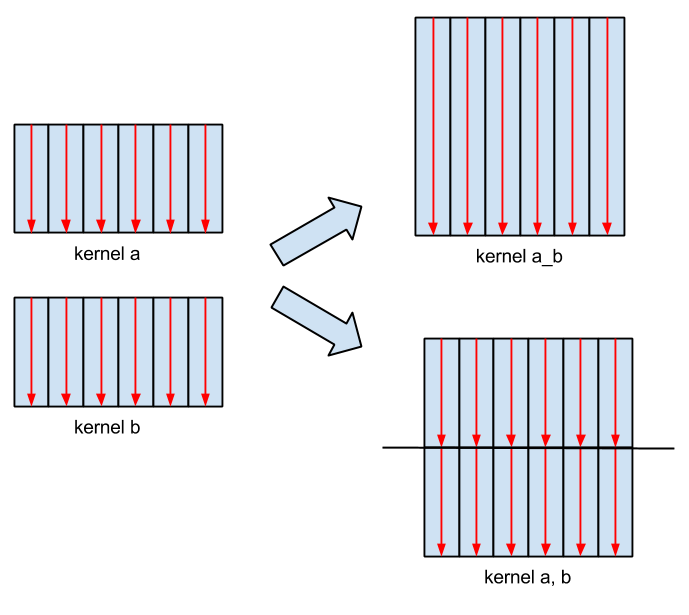
\includegraphics[width=15cm]{img/kernel-fusion.png}
\caption{kernel fusion}
\label{fig:my_label1}
\end{figure}

\section{Halide schedule compute\_at}
    Halide provide a schedule named “compute\_at”, and it can fuse multiple kernels into one kernel. The schedule uses the second way, doing redundant works to calculate the data needed itself. The main disadvantage of this way is, the more the kernels fused, the more the redundant works shows.

    For example, Figure~\ref{fig:my_label2} shows the pixels accessed to calculate one pixel’s result. The pink part represents the pixels accessed in the kernel.The algorithm is to obtain the pixel on the target pixel’s left and right, and calculate the sum of the two pixels and the target pixel. The example shows processing the image using the algorithm two times. We can see every kernel access two extra pixels except the target pixel.
	
\begin{figure}[hbtp]
\centering
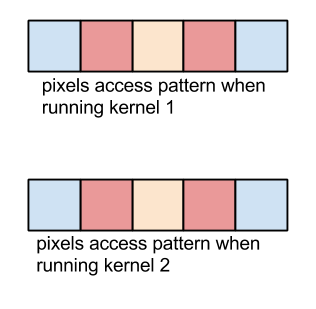
\includegraphics[width=8cm]{img/figure2.png}
\caption{accessing pattern of 2 kernels}
\label{fig:my_label2}
\end{figure}

    Figure~\ref{fig:my_label3} shows the calculating flow of doing one dimension blur algorithm twice, and applying kernel fusion by doing redundant works. We can see the number of pixels accessed are five in the first kernel, and three in the second kernel.
	
\begin{figure}[hbtp]
\centering
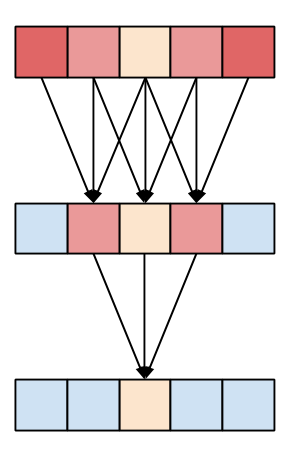
\includegraphics[width=8cm]{img/figure3-6(for-paper).png}
\caption{Example of the calculating flow when doing redundant works}
\label{fig:my_label3}
\end{figure}
	
    Figure~\ref{fig:my_label4} shows the pixels accessed to calculate one pixel’s result if we use Halide schedule, compute\_at. The pink part represents pixels accessed in the first kernel. The burgundy part represents the extra pixels accessed in the second kernel. We can see if we want to eliminate the dependency without barrier, we need to access two extra pixels than original.
	
\begin{figure}[hbtp]
\centering
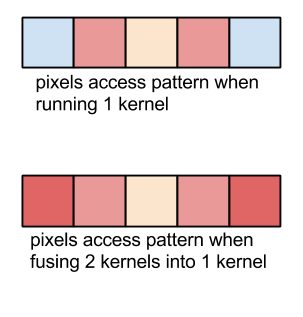
\includegraphics[width=8cm]{img/figure3.png}
\caption{accessing pattern of compute\_at}
\label{fig:my_label4}
\end{figure}
	
    Figure~\ref{fig:my_label5} shows the accessing pattern using kernel fusion when processing an image with a blur algorithm accessing the 8 pixels around the target pixel. The pink part represents pixels accessed in the first kernel. The burgundy part represents the extra pixels accessed in the second kernel. We can see when blurring the image 2 times, the increasing redundant works are to calculate 16 pixels compared to the original version. And the redundant works will be calculating 24 pixels compared to only fuse 2 kernels into one if we fuse 3 kernels into one kernel. So the redundant works grow fast according to how many kernels we fuse.

\begin{figure}[hbtp]
\centering
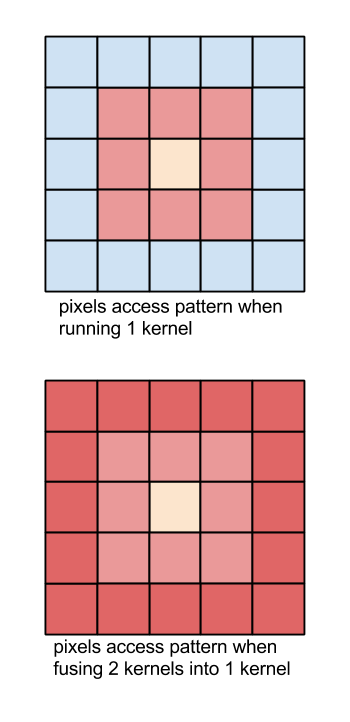
\includegraphics[width=10cm]{img/figure4.png}
\caption{accessing pattern of compute\_at 2}
\label{fig:my_label5}
\end{figure}

\section{Approach: enqueue\_kernel}
    We implement our enqueue\_kernel feature on an Open-Source Project - POCL (Portable Computing Language.) It is an OpenCL implementation. Our approach will help the user to branch to the new kernel at runtime by using the “block” which is defined by the Clang\cite{clangori} (a compiler front end for the C, C++, Objective-C and Objective-C++ programming languages) and it can be used like a function pointer. According to the OpenCL 2.0 spec, enqueue\_kernel’s second input argument is “kernel\_enqueue\_flags\_t flags”. The flags can be CLK\_ENQUEUE\_FLAGS-\_NO\_WAIT, CLK\_ENQUEUE\_FLAGS\_WAIT\_KERNEL and CLK\_ENQUEUE\_FLA-
GS\_WAIT\_WORK\_GROUP.

    Figure~\ref{fig:my_label6} is a flowchart presenting our approach. We implement our approach pre-parser inside the host OpenCL API clCreateProgramWithSource. When the kernel source code are input, our pre-parser will process the source code according to which flag is specified.

    Our approach can perform full functionality of the last flag mentioned, but leave the first and the second flag limited functionality. We add a pre-parser before compiling the kernel source code to binary program (before clCreateProgramWithSource.) to do setup for the enqueue\_kernel function according to the kernel\_enqueue\_flags\_t. 
	
\begin{figure}[hbtp]
\centering
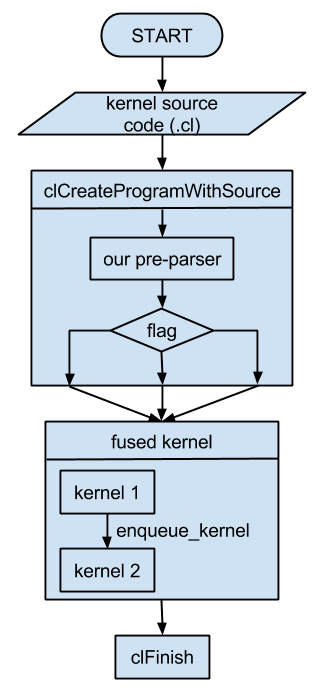
\includegraphics[width=10cm]{img/overview-approach.png}
\caption{Flowchart of approach}
\label{fig:my_label6}
\end{figure}

    If the last flag is specified, we will switch the enqueue command to the last line of the kernel. And then branch to the new kernel using block. This will let all work items within a work group wait for all work items to finish their previous kernel, and then branch to the new kernel by block.
    If the second flag is specified, we will switch the enqueue command to the last line with a barrier before it. But this will not let all work group wait for the others to finish the previous kernel, since synchronization between work groups cannot be done using OpenCL currently.
    If the first flag is specified, we will immediately branch to the new kernel by block. So the current kernel will be blocked and wait for the new kernel to finish. But the full functionality of the first flag should be enqueueing the new kernel, and then create a new thread for the new kernel. So the new kernel and the current kernel can be running at the same time. This will give the process better performance than our approach. But the first flag won’t be used when performing kernel fusion. The new kernel should have no dependency with the original kernel, since they should run at the same time.
	
\section{Comparison between two features}
    Besides Halide schedule “compute\_at” need to do redundant works, while our approach may not need to, one more difference is that our approach supports deciding which kernel to be fused at runtime. This can be used to perform dynamic kernel fusion while Halide schedule “compute\_at” can not. Halide schedule compute\_at need to decide which kernel to be fused at compile time, and Halide CodeGen will generate the corresponding OpenCL host and device source code.

\section{Different Approach: enqueue\_kernel}
    According to the original OpenCL 2.0 spec, there are some more built-in functions, host CL APIs, helper functions and data type definitions that need to be supported. Including host CL APIs clCreateCommandQueueWithProperties, built-in function get\_default\_queue. 
    clCreateCommandQueueWithProperties can be used to create a command queue with different properties supported. Since with different kernel enqueued, we may need command queue with different properties. The properties will be stored as a list. And the get\_default\_queue built-in function will be used to get the default device queue during the kernel (device queue is supposed to be the default command queue, in order to put the new enqueue kernel command into the default command queue.) 
	
    By using the host API clCreateCommandQueueWithProperties and the built-in function get\_default\_queue, we can put the kernel which we want to enqueue in the current kernel into the default command queue which we can obtain from get\_default\_queue and then enqueue it through the OpenCL command queue feature.
	
    But the difficulty here is, according to the OpenCL 2.0 spec, the enqueue\_kernel built-in function’s input argument is “block” which is defined by the Clang\cite{clangori} (a compiler front end for the C, C++, Objective-C and Objective-C++ programming languages.) It can be used like a function pointer, so we can not directly obtain the kernel name mapping to this block. But in POCL, we need to first create the whole program by clCreateProgramWithSource to create the binary. It will be compiled to .bc through LLVM (Low Level Virtual Machine), and then being compiled to .so. To enqueue a kernel, we need its kernel name to search for the code section in the .so file. The enqueue command in the command queue should contain the kernel name, which we currently do not have.
	
\section{Temporary storage allocation}
    To use enqueue\_kernel, we will need to allocate temporary storage. Since the output of the previous kernel will be the input of the next kernel, we need a temporary storage to store these data for the next kernel to read them. The storage type should be declared global, so all work items within all work groups can read it.

    We will need to allocate temporary storage at the host source code, and use allocated temporary storage instead of the original storing destination at the kernel source code.

\chapter{Experiments}
\quad \  \ We test the framework with two different application – Bilateral\cite{bilateral} and Local Laplacian\cite{locallaplacian} which are Halide example with tuned schedule for CPU and GPU at three different platform including android platform (Nexus 7) ,detail platform information is shown as table ~\ref{platform1}~\ref{platform2} ,we got at most 57\% improvement with static dispatch and dynamic dispatch compared to best single device. 

\begin{table}[]
\centering
\caption{Test Platform Hardware information}
\label{platform1}
\begin{tabular}{|l|l|l|}
\hline
Platform & CPU & GPU \\ \hline
Android Nexus 7 & \begin{tabular}[c]{@{}l@{}}Quad-core\\ 1.5 GHz Krait\end{tabular} & \begin{tabular}[c]{@{}l@{}}Adreno\\ 320\end{tabular} \\ \hline
PC 1 & \begin{tabular}[c]{@{}l@{}}Intel(R) Core(TM)\\  i5-4590 CPU @ 3.30GHz\end{tabular} & \begin{tabular}[c]{@{}l@{}}ATI Radeon\\ R7 260X\end{tabular} \\ \hline
PC 2 & \begin{tabular}[c]{@{}l@{}}Intel(R) Core(TM)\\  i5-3470 CPU @ 3.20GHz\end{tabular} & \begin{tabular}[c]{@{}l@{}}NVIDIA\\ GTX 750\end{tabular} \\ \hline
\end{tabular}
\end{table}

\begin{table}[]
\centering
\caption{Test Platform software information}
\label{platform2}
\begin{tabular}{|l|l|l|}
\hline
Platform & Compiler & OpenCL Runtime \\ \hline
Android Nexus 7 & \begin{tabular}[c]{@{}l@{}}Android Ndk r10c\\ Halide release\_2015\_06\_03\end{tabular} & Adreno driver for nexus 7 \\ \hline
PC 1 & \begin{tabular}[c]{@{}l@{}}Clang++ 3.6\\ Halide release\_2015\_06\_03\end{tabular} & AMD APP SDK 3.0 Beta \\ \hline
PC 2 & \begin{tabular}[c]{@{}l@{}}Clang++ 3.6\\ Halide release\_2015\_06\_03\end{tabular} & Nvidia driver 337 \\ \hline
\end{tabular}
\end{table}



At the beginning, we have to prove that it is possible we can improve performance by split work into two partitions. So we took Bilateral and Local Laplacian as our benchmark, in each case we gave same input and try to make halide to compute partial output from 10\% to 90\% on CPU and GPU to show the relationship between execution time and workload. 
\begin{figure}[hbtp]
\centering
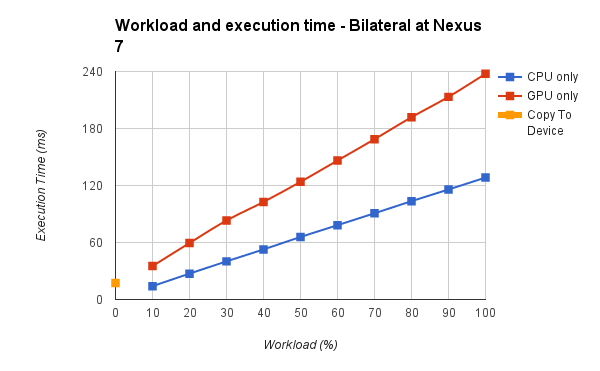
\includegraphics[width=12cm]{img/Result-WorkloadbetweenCPUandGPU(Bilateral@Nexus7).png}
\caption{Result-Bilateral at Nexus 7 }
\label{fig:my_label}
\end{figure}

\begin{figure}[hbtp]
\centering
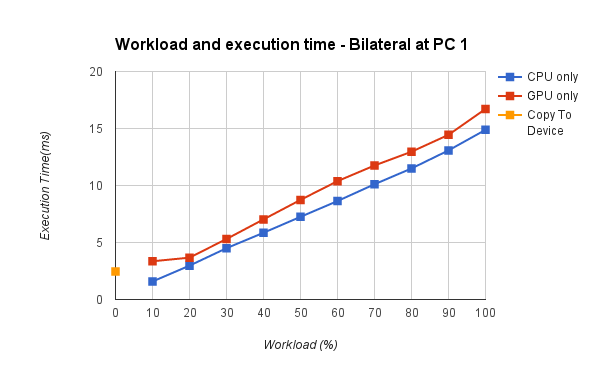
\includegraphics[width=12cm]{img/Result-WorkloadbetweenCPUandGPU(Bilateral@PC1).png}
\caption{Result-Bilateral at PC 1 }
\label{fig:my_label}
\end{figure}

\begin{figure}[hbtp]
\centering
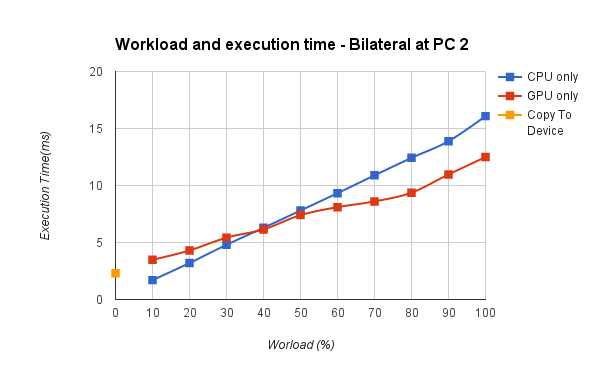
\includegraphics[width=12cm]{img/Result-WorkloadbetweenCPUandGPU(Bilateral@PC2).png}
\caption{Result-Bilateral at PC 2 }
\label{fig:my_label}
\end{figure}

According to experiment result we got, we notice that we could improve performance by split workload into two different devices when processing Bilateral filter. 

%We also test another filter local laplacian the relation between workload and execution time. 
\begin{figure}[hbtp]
\centering
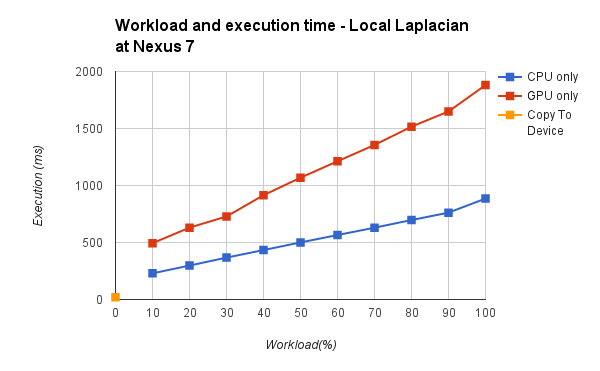
\includegraphics[width=12cm]{img/Result-WorkloadbetweenCPUandGPU(LocalLaplacian@Nexus7).png}
\caption{Result-Loca lLaplacian at Nexus 7 }
\label{fig:my_label}
\end{figure}

\begin{figure}[hbtp]
\centering
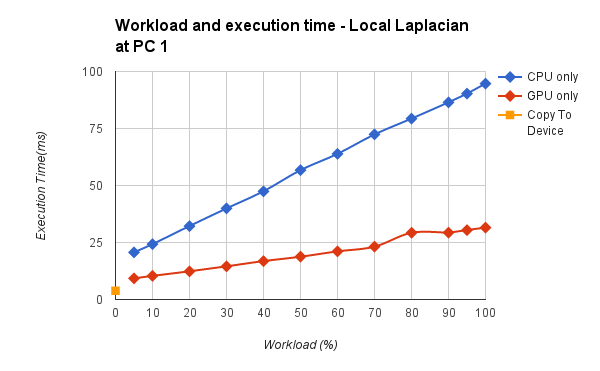
\includegraphics[width=12cm]{img/Result-WorkloadbetweenCPUandGPU(LocalLaplacian@PC1).png}
\caption{Result-Local Laplacian at PC 1 }
\label{fig:my_label}
\end{figure}

\begin{figure}[hbtp]
\centering
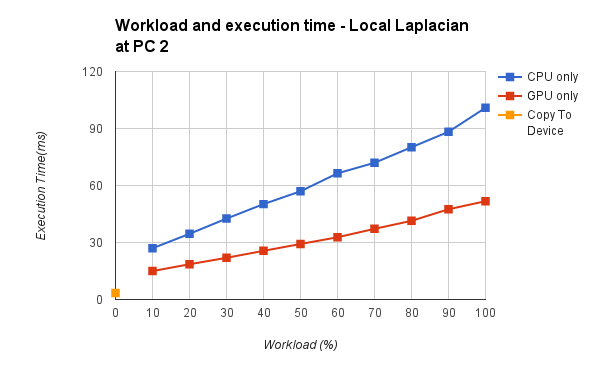
\includegraphics[width=12cm]{img/Result-WorkloadbetweenCPUandGPU(LocalLaplacian@PC2).png}
\caption{Result-Local Laplacian at PC 2 }
\label{fig:my_label}
\end{figure}

We notice that the trend line of Local laplacian is similar to Bilateral. However, there is one little part which is different to Bilateral, that is, according to the trend line, when the workload of bilateral filter equals to zero, the execution time of CPU also equals to zero and the execution time of GPU would equal to the time of copying to device, but the trend line of Local laplacian is not, the trend line of CPU will be higher than zero when the workload equals to zero  and the trend line of GPU will also be higher than the time of coping to device, which means if we split work of local laplacian into 2 or more partition the execution of two or more partition will greater than only 1 partition and it will increase when we split work into more partition, which also implies that we may not get same improvement between static dispatch and dynamic dispatch when the framework handling the case like local laplacian.

\section{Static Dispatch}

\quad \ \ To test static dispatch we assign different workload to CPU and GPU to test the best performance on Static Dispatch. Totally, there are 9 composition between CPU and GPU workload.

In those results, the high peak of the CPU workload and the mapping GPU workload (GPU workload reverse in the diagram) should be the ideal execution time of static dispatch and the line is the real execution time of static dispatch. We got about 1.21x , 1.55x and 1.16x at Nexus7, PC 1 and PC2 respectively when processing bilateral filter compared to best single device. We also got 1.24x, 1.03x and 1.11 speedup improvement at Nexus7, PC 1 and PC2 respectively  when processing Local Laplacian filter compared to best single device. 

However, in the diagrams of Bilateral filter, the static dispatch (the line) is higher than the peak. The gap between high peak and the real static execution time should be overhead of OpenCL runtime, we will profile and discuss the runtime information on next section.

\begin{figure}[hbtp]
\centering
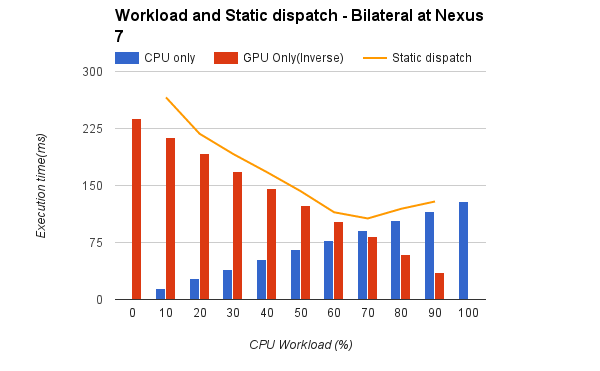
\includegraphics[width=12cm]{img/Result-WorkloadAndStaticDispatch(Bilateral@Nexus7)}
\caption{Result- Bilateral at Nexus 7 }
\label{fig:my_label}
\end{figure}

\begin{figure}[hbtp]
\centering
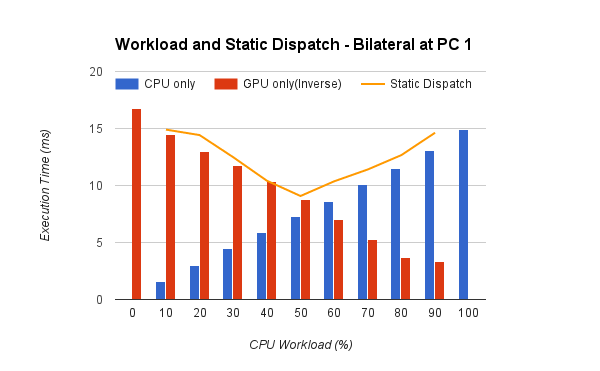
\includegraphics[width=12cm]{img/Result-WorkloadAndStaticDispatch(Bilateral@PC1)}
\caption{Result- Bilateral at PC 1 }
\label{fig:my_label}
\end{figure}

\begin{figure}
\centering
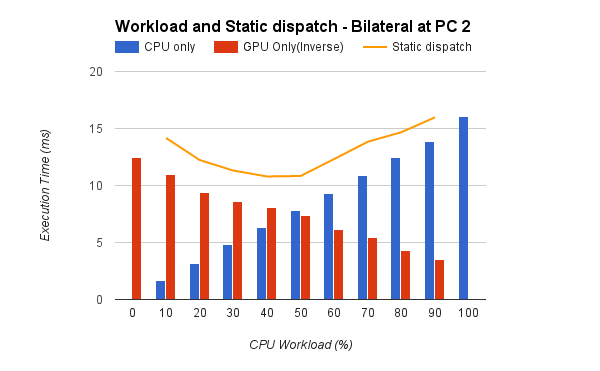
\includegraphics[width=12cm]{img/Result-WorkloadAndStaticDispatch(Bilateral@PC2)}
\caption{Result- Bilateral at PC 2 }
\label{fig:my_label}
\end{figure}


\begin{figure}[hbtp]
\centering
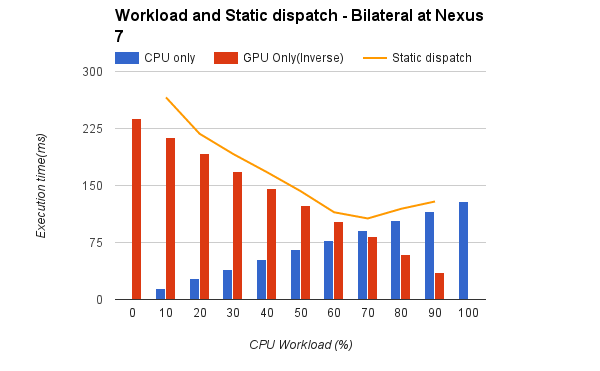
\includegraphics[width=12cm]{img/Result-WorkloadAndStaticDispatch(Bilateral@Nexus7)}
\caption{Result- Local Laplacian at Nexus 7 }
\label{fig:my_label}
\end{figure}

\begin{figure}[hbtp]
\centering
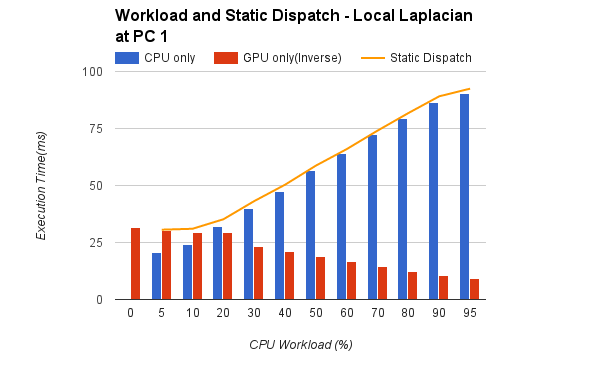
\includegraphics[width=12cm]{img/Result-WorkloadAndStaticDispatch(LocalLaplacian@PC1)}
\caption{Result- Local Laplacian at PC 1}
\label{fig:my_label}
\end{figure}

\begin{figure}[hbtp]
\centering
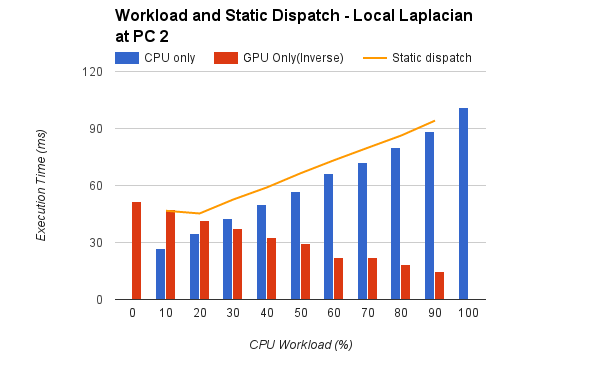
\includegraphics[width=12cm]{img/Result-WorkloadAndStaticDispatch(LocalLaplacian@PC2)}
\caption{Result- Local Laplacian at PC2 }
\label{fig:my_label}
\end{figure}

\section{Dynamic Dispatch}
\quad \  \ After implement static dispatch, we want to implement an easier way to programmer to use both devices, we also implement dynamic dispatch and hope it could be effective as static dispatch.

\begin{figure}[!hbtp]
\centering
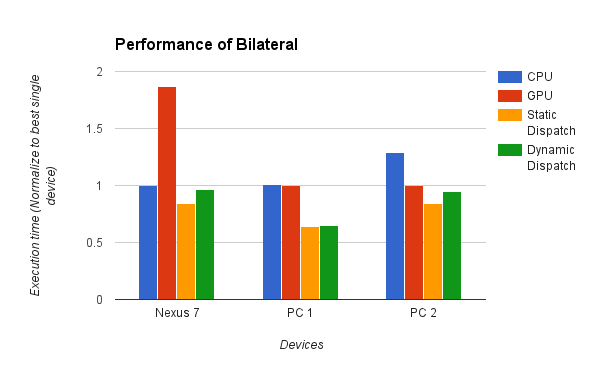
\includegraphics[width=12cm]{img/PerformanceOfBilateral.png}
\caption{Performance of Bilateral filter. For each devices, execution time is shown normalized to the best performing single device – CPU-only or GPU-only.}
\label{fig:my_label}
\end{figure}

\begin{figure}[!hbtp]
\centering
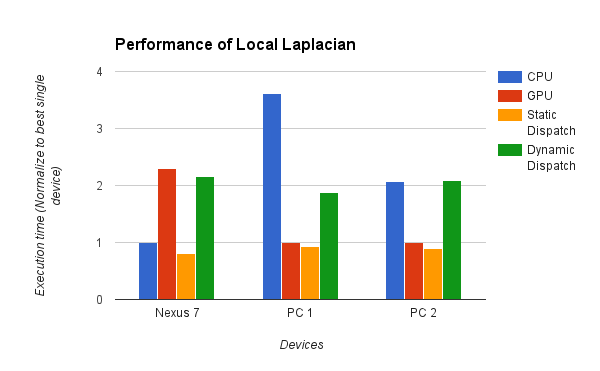
\includegraphics[width=12cm]{img/PerformanceOfLocalLaplacian.png}
\caption{Performance of Local Laplacian  filter. For each devices, execution time is shown normalized to the best performing single device – CPU-only or GPU-only.}
\label{fig:my_label}
\end{figure}

According to the results, it shows that dynamic dispatch will be slower than static dispatch especially when processing filter like local laplacian which matchs our assumption before. It is because filter like local laplacian which will refer to all input data cannot split into multiple blocks or it will refer to all input redundantly. 

\section{Profile OpenCL Runtime information}

\quad \  \ The gap between ideal static execution real static execution should be the overhead of OpenCL runtime information.To prove that, we profile OpenCL runtime information to figure out the bottleneck of our framework. We profile the runtime information of GPU only with processing specific percentage workload and static dispatch with same workload to compare the execution of each stage of OpenCL API.


\begin{figure}[!hbtp]
\centering
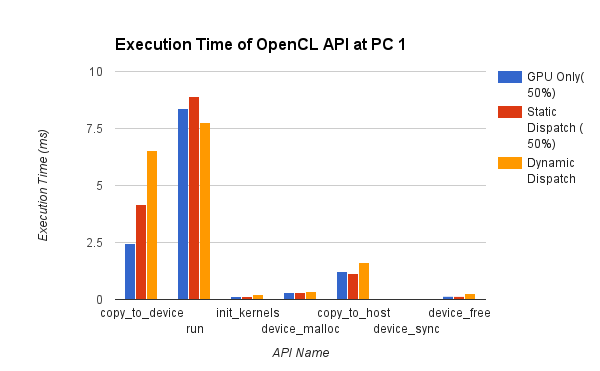
\includegraphics[width=12cm]{img/ExecutionTimeOfAPI(Bilateal@PC1).png}
\caption{Execution time Of OpenCL API at PC1 each API is normalized to GPU only.}
\label{fig:my_label}
\end{figure}

\begin{figure}[!hbtp]
\centering
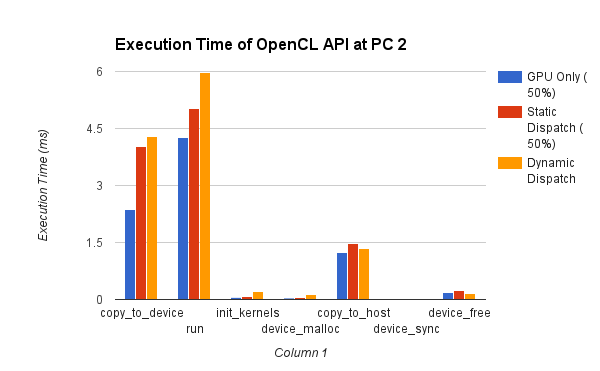
\includegraphics[width=12cm]{img/ExecutionTimeOfAPI(Bilateal@PC2).png}
\caption{Execution time Of OpenCL API at PC2 each API is normalized to GPU only.}
\label{fig:my_label}
\end{figure}

\section{CUDA and OpenCL}
\quad \  \ In addition to OpenCL, Halide also support CUDA as the language of GPU which means our framework should also support CUDA, so we also measured the performance and make a comparison between CUDA and OpenCL when processing bilateral and local laplacian at PC2.



\begin{figure}[hbtp]
\centering
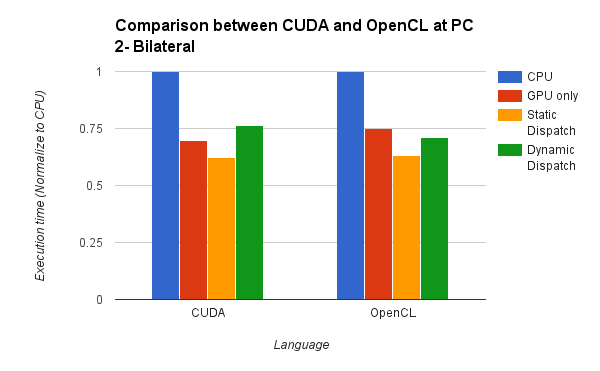
\includegraphics[width=12cm]{img/ComparisonBetweenCUDAAndOpenCL(Bilateral).png}
\caption{Comparison between CUDA and OpenCL when processing Bilateral Filter. Each time is normalized to CPU execution time}
\label{fig:my_label}
\end{figure}

\begin{figure}[hbtp]
\centering
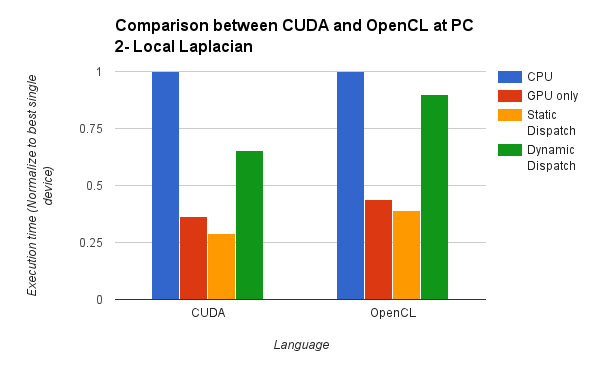
\includegraphics[width=12cm]{img/ComparisonBetweenCUDAAndOpenCL(LocalLaplacian).png}
\caption{Comparison between CUDA and OpenCL when processing Local Laplacian Filter. Each time is normalized to CPU execution time}
\label{fig:my_label}
\end{figure}

\section{Different Input Size}
\quad \  \ To test the influence of different input size, we also experiment different input with 8192*6960 pixel.According to our results, PC 1 can similar to our predict execution time, however, PC 2 still slower to our predict execution time even if we enlarge input size .To figure out the reason, we also profile the API time of this input size, in next section, we will discuss the results.

\begin{figure}[!hbtp]
\centering
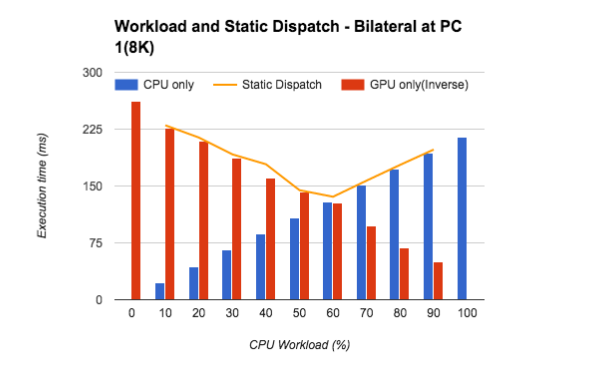
\includegraphics[width=12cm]{img/WorkloadAndStaiticDispatch-BilateralAtPC1(8K).png}
\caption{Result- Bilateral at PC 1 with 8K input size}
\label{fig:my_label}
\end{figure}

\begin{figure}[!hbtp]
\centering
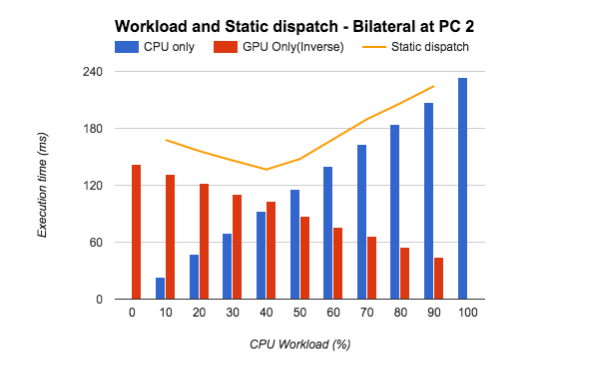
\includegraphics[width=12cm]{img/WorkloadAndStaiticDispatch-BilateralAtPC2(8K).png}
\caption{Result- Bilateral at PC 2 with 8K input size}
\label{fig:my_label}
\end{figure}


\section{OpenCL API exection time with larger size}
\quad \  \ After profiling OpenCL API execution time, Figure ~\ref{fig:ExeTime8KPC2} shows that the gap between GPU only and static dispatch still exists in PC 2 when input size became to 8192*6960.

\begin{figure}[!hbtp]
\centering
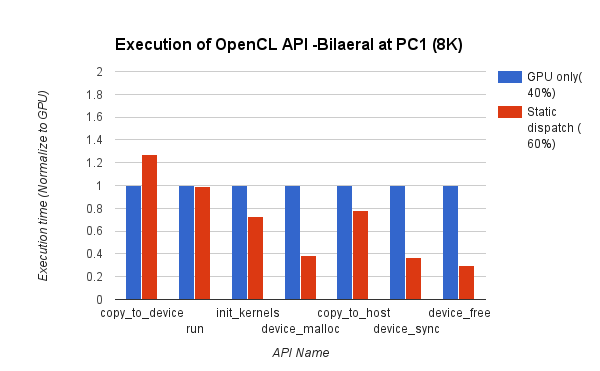
\includegraphics[width=12cm]{img/ExecutionofOpenCLAPI-BilateralatPC1(8K).png}
\caption{Execution time of openCL API - Bilateral at PC 1 (8K)}
\label{fig:ExeTime8KPC1}
\end{figure}

\begin{figure}[!hbtp]
\centering
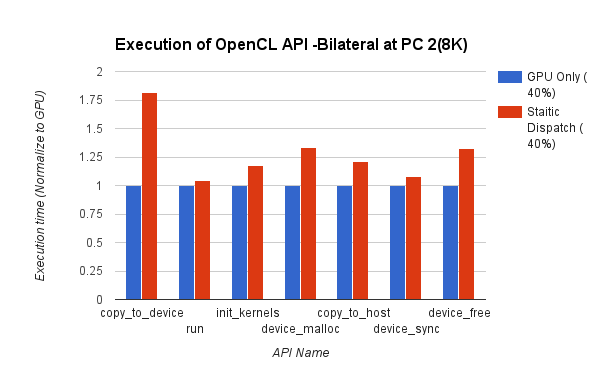
\includegraphics[width=12cm]{img/ExecutionofOpenCLAPI-BilateralatPC2(8K).png}
\caption{Execution time of openCL API - Bilateral at PC 2 (8K)}
\label{fig:ExeTime8KPC2}
\end{figure}




\chapter{Future Work}
    For the future work, we have three things to do. First, we should add our enqueue\_kernel approach to Halide OpenCL CodeGen and add automatic temporary storage allocation and using them in the kernel source code which we generated. This should improve the OpenCL performance of Halide.

    Second, we need to add temporary storage allocation into Halide OpenCL CodeGen, including OpenCL host source code and kernel source code. Since we need to do allocation at the host part, and change the usage and storing destination to our new allocated temporary storage at the kernel part.

    Last, we should implement full functionality of enqueue\_kernel with the first flag mentioned, CLK\_ENQUEUE\_FLAGS\_NO\_WAIT. This will offer us a new way to improve performance, because we can separate the works that have no dependency issues, and then enqueue a new kernel for these works. And we should also implement full functionality of CLK\_ENQUEUE\_FLAGS\_WAIT\_KERNEL, thus we can use enqueue\_kernel more flexibly and can make sure all work group finish the previous kernel.

\chapter{Conclusion}
Our work is to make framework which is easy to use and can get improvement by using synergistic computation. In this paper, we use Halide as our language and make a runtime on Halide to build a synergistic and easy computing environment. 
According to our experiment, we could improve the execution time by splitting the workload into 2 or more partitions and dispatching them to CPU and GPU.  Also, our framework could get at most 1.55x speedup when processing case like Bilateral compared to fastest single device, but when processing algorithm like local laplacian we can get only few improvement when using static dispatch and may not get improvement when using dynamic dispatch because of the feature of the algorithm. However, even if we can get at most 1.55x speedup improvement, we still cannot get ideal performance improvement which we predict. But when kernel computing takes more percentage in the whole execution, in other word, when the algorithm become more complex, we could reduce the influence of OpenCL runtime and get more improvement.
In short, with the feature of Halide, we build a synergistic computing environment that is easy to program, tune performance and take advantage of both CPU and GPU to computing the jobs.


%\appendix

\backmatter

\addcontentsline{toc}{chapter}{\bibname}
\bibliographystyle{unsrt}

% Your bibliography goes here
\nocite{*}
\bibliography{thesis}

\end{document}

